\documentclass[aps,pre,twocolumn,superscriptaddress,showpacs]{revtex4-1}
%
%==================================================================
% PREFACE
%==================================================================
%
% BibTeX
\bibliographystyle{apsrev}
\bibliographystyle{plain}
%
%Packages
\usepackage{natbib}
\usepackage[english]{babel}
\usepackage[dvips]{graphics}
\usepackage{graphicx,epsfig}
\usepackage{amsmath}
\usepackage{color}
\usepackage{float}
\usepackage{multirow}
\usepackage[normalem]{ulem}
\usepackage{booktabs}
\usepackage{amsfonts} 
\usepackage{multirow}
\usepackage{subcaption}
\usepackage{braket}

%\allowdisplaybreaks

\newcommand{\om}{\omega}
\newcommand{\omx}{\omega_1}
\newcommand{\omy}{\omega_2}
\newcommand{\En}{\mathcal{E}_n}
\newcommand{\abinitio}{\textit{ab initio }}

%Text commands
\newcommand{\CR}[1]{{\color{red}{#1}}}
\newcommand{\CB}[1]{{\color{blue}{#1}}}
\newcommand{\CG}[1]{{\color{green}{#1}}}
\newcommand{\no}[1]{{\sout{\color{red}{#1}}}}
\newcommand{\nob}[1]{{\sout{\color{blue}{#1}}}}
\newcommand{\bfeq}[1]{{\boldsymbol{#1}}}

\begin{document}
\title{Theoretical calculations of the Inelastic Confinement-Induced Resonances and its asymmetric splitting of two ultracold atoms trapped in optical lattices}
%
\author{T. S\'anchez-Pastor}
\affiliation{Grupo de Sistemas Complejos,
Escuela T\'ecnica Superior de Ingenier\'ia Agron\'omica,
Alimentaria y de Biosistemas,
Universidad Polit\'ecnica de Madrid,
Avda. Puerta de Hierro 2-4, 28040 Madrid, Spain.}

\author{F. Revuelta}
\affiliation{Grupo de Sistemas Complejos,
Escuela T\'ecnica Superior de Ingenier\'ia Agron\'omica,
Alimentaria y de Biosistemas,
Universidad Polit\'ecnica de Madrid,
Avda. Puerta de Hierro 2-4, 28040 Madrid, Spain.}

\author{Alejandro Saenz}
\affiliation{AG Moderne Optik, 
Institut für Physik, 
Humboldt-Universität zu Berlin, 
Newtonstrasse 15, 12489 Berlin, Germany.}
%
%------------------------------------------------------------------------------------
\begin{abstract}
	In this work we study several aspects of the Inelastic CIR caused by the coupling of center-of-mass and relative motion for a system of two Lithium 		ultracold atoms in anharmonic sextic traps. We take advantage of the \abinitio calculations to ensure the CRC model robustness presented in [Phys. 	Rev. Lett. \textbf{109} 073201 (2012)] computing the exact trap relative motion energy of the resonance. The last study assumed the resonance to occur 	at a energy distance of $\hbar \omega_z$ above the free trap state limit which is in disagreement with this approach, where we found a correct value of 	$0.8\hbar \omega_z$. Furthermore, we show that in 3-D confinements the approximation is not valid as well as the theory used to compute the 		resonance positions. Finally, we describe in depth the origin of the asymmetric splitting of the Inelastic CIRs for increasing values of the trap anisotropy.
\end{abstract}
%------------------------------------------------------------------------------------
%\pacs{05.45.-a, 33.20.Tp, 82.20.-w}

\maketitle

%------------------------------------------------------------------------------------
\section{Introduction}  \label{sec:intro}
	Contar un poco de historia de la observación de este tipo de resonancias, por qué los sistemas ultrafríos están de moda (control) y resonancias de 		Feshbach (cambiar B es cambiar a). Acoplamiento CM-rm como causante de los cruces evitados, transiciones no adiabáticas y rmacionarlo con el 		teorema adiabático.
%------------------------------------------------------------------------------------
\section{Two-atom numerical simulations}  \label{sec:system}
	\subsection{Hamiltonian}
		The system is formed by two Lithium ultracold atoms that interact only via s-wave scattering due to the extremely low temperature of the gas 			leading to a spatial symmetry where rm and CM coordinates reduced the complexity of the calculations. Relative motion distance is defined as			$\bfeq{r} = \bfeq{r_1} - \bfeq{r_2}$ whereas CM coordinate as $\bfeq{R} = \frac{1}{2}(\bfeq{R_1} + \bfeq{R_2})$. The Hamiltonian is then given by:
		
		\begin{eqnarray}
			\mathcal{H}(\bfeq{r}, \bfeq{R}) &=& T_{CM}(\bfeq{R}) + T_{rm}(\bfeq{r}) + V_{CM}(\bfeq{R}) + 				\nonumber \\ 
			 &+& V_{rm}(\bfeq{r}) + W(\bfeq{r}, \bfeq{R}) + U_{int}(|\bfeq{r}|), 
			 \label{eq:Hamiltonian}
		\end{eqnarray}
		
		where the $T$'s are the kinetic energy operators and the $V$'s the separable potential energies for both rm and CM coordinates, while $W$ 		accounts for the rm-CM coupling, which is nonzero for anharmonic traps and for homonuclear systems. The coupling term is responsible of 			the avoided crossings and therefore of the Inelastic CIRs. $U_{int}$ is the particle-particle potential energy often described in analytic derivations by 		the pseudopotential $U_{int} = \frac{4\pi \hbar^2 a_s}{m} \delta(\bfeq{r})\frac{\partial}{\partial \bfeq{r}}$, where $a_s$ is the 3-D s-wave scattering length.
		
		In a 3-dimensional optical trap the potential terms are
		\begin{eqnarray}
			V_{rm}(\bfeq{r}) &=& 2 \sum_{j=x,y,z} V_j \sin^2 \left(\frac{1}{2}k r_j \right), \\
			V_{CM}(\bfeq{R}) &=& 2 \sum_{j=x,y,z} V_j \sin^2 \left(k R_j \right), \\
			W(\bfeq{r}, \bfeq{R}) &=& -4 \sum_{j=x,y,z} V_j \sin^2 \left(\frac{1}{2}k r_j \right) \sin^2 \left(k R_j \right).
		\end{eqnarray}
		
		$k$ is the angular wavenumber and $V_j$ is the potential depth in any direction. Associated with the potential depth, the trap frequency are 			$\omega_j = k_j\sqrt{\frac{2V_j}{m}}$ and the characteristic trap length $d_j = \sqrt{\frac{2\hbar}{m\omega_j}}$. Thus, the anisotropies can be 			defined in units of the transversal component: $\eta_j = \frac{\omega_j}{\omega_y}$.
	
	
	\subsection{Ab Initio calculations}
		Schrödinger equation is solved using the full six-dimensional Hamiltonian of eq.(\ref{eq:Hamiltonian}) in spherical coordinates. The exact 				diagonalization is carried using realistic short-range interatomic potentials: numerically Born-Oppenheimer curves. The interaction potential is then 		varied to tune the scattering length. Regarding the trap potential we expand to sixth order to account for anisotropies associated with non-vanishing 		coupling terms.  We use a basis set of B-splines and spherical harmonics for the angular dependencies. \cite{PhysRevA.84.062710}
		
		The computation of the eigenenergies and eigenfunctions is obtained in a two-step method as follows: (i) First, the separable part of the 				Hamiltonian is diagonalized in order to compute the eingenfunctions $\ket{\psi^{rm}_n}$ and $\ket{\Psi^{CM}_{\bfeq{m}}}$, which will be called 			\textit{orbitals} because of their similarity with the electronic orbitals used in Quantum Chemistry. (ii) The coupling remaining coupling term is solved 		building a new basis. The states of this basis are the so-called \textit{configurations} $\ket{\Phi_{n, \bfeq{m}}} = \ket{\psi^{rm}_n \Psi^{CM}_{\bfeq{m}}}$. 
		
		Ab initio calculations are used to compute the dependence of the eigenenergies with the scattering length for a wide range of anisotropies $\eta_x$. 
		The middle points of the avoided crossings are the positions of the Inelastic CIR that we compare with the theory predictions.
		
		
%------------------------------------------------------------------------------------
\section{Improving Inelastic CIR calculations}  \label{sec:theory}
Introducción contando en profundidad el origen de las ICIR, la aproximación de Simón y lo de la C.

\subsection{3-D}
jjejejeje

	\begin{figure}[h]
   	 \centering
    	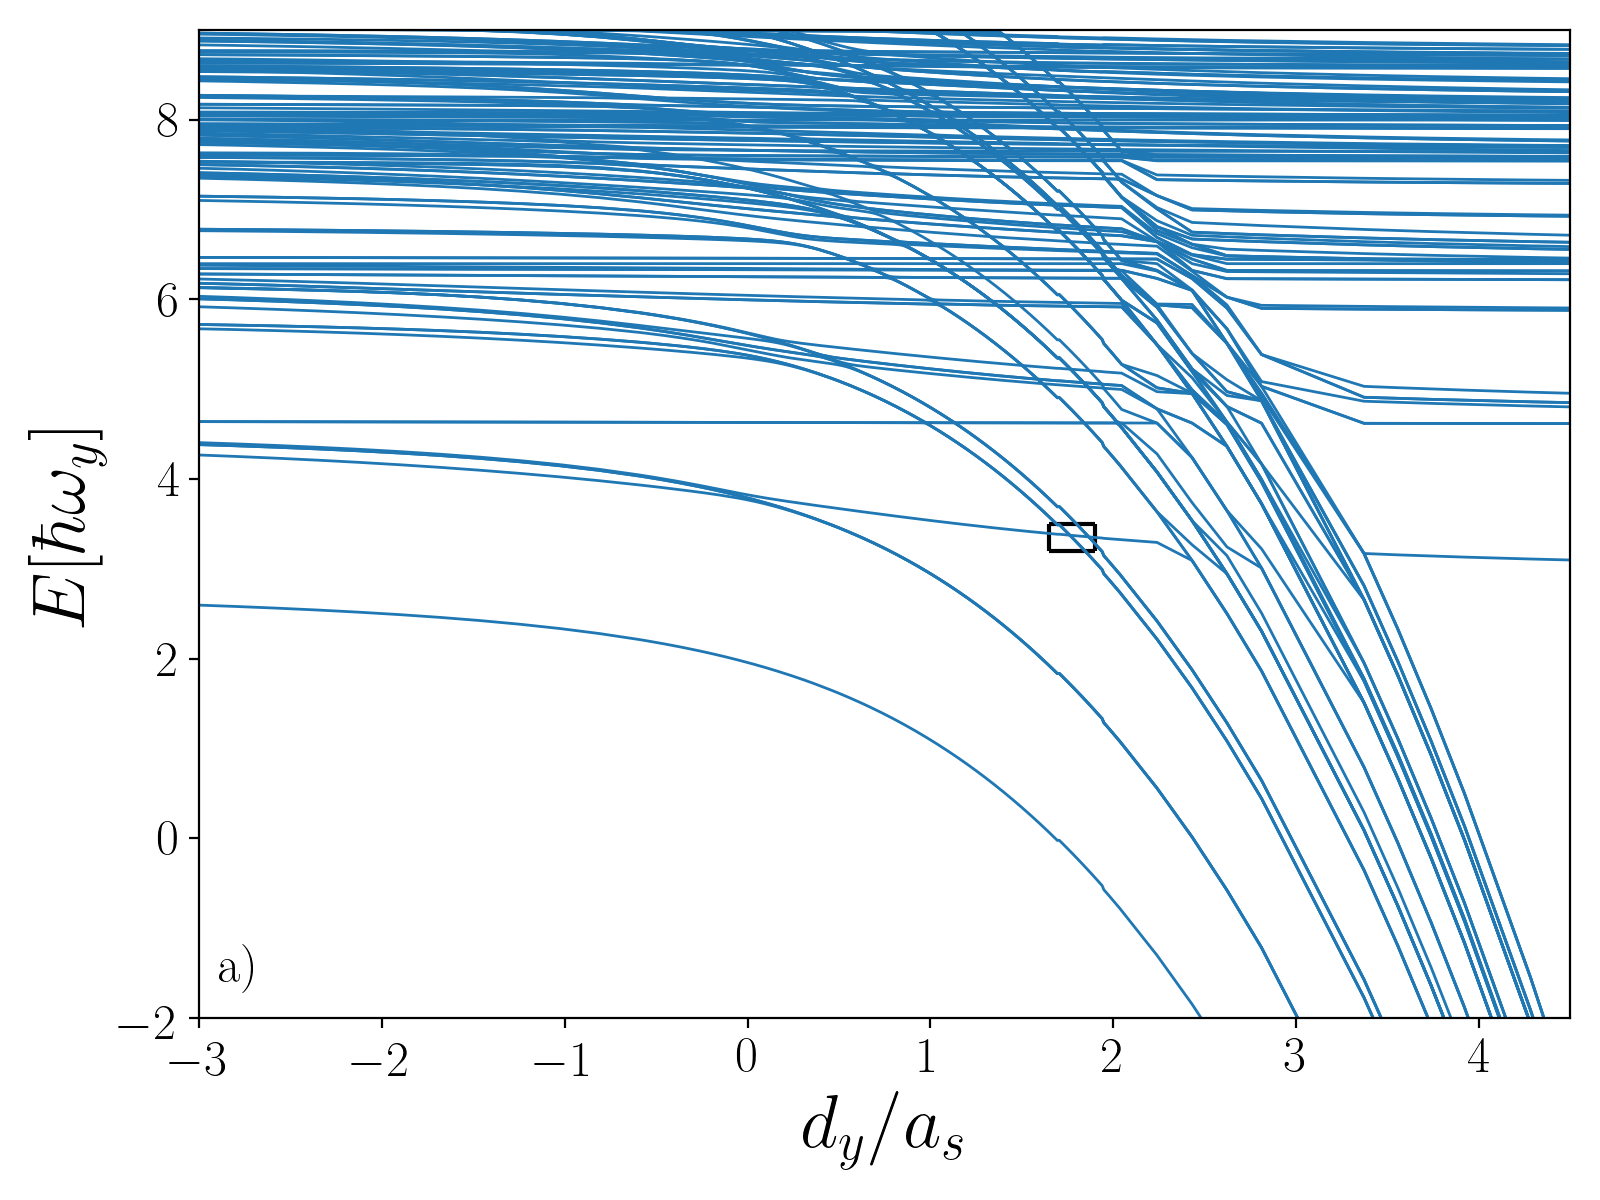
\includegraphics[scale=0.30]{/Users/tomy/PhD/Ultracold_Atoms_src/Analysis/q3d/Results/Figures/Ix4993_Iy4993_Iz4993_Easc_solid.png}
    	\caption{Adiabatic Spectrum of the full coupled Hamiltonian for $^7$Li atoms confined in an isotropic sextic trapping potential with $V_x = V_y = V_z = 35.9E_r$, $\eta_x = \eta_y = 1$ and $\lambda=1000$ nm. All states bending down to $-\infty$ are molecular states originating from the rm bound state $\psi^{(b)}$ with different CM excitations, whereas the states remaining constant are trap states of different rm excitations $\psi^{1}$ and zero CM excitations.}
    	\label{fig:3D spectrum}
	\end{figure}
	
	\begin{figure}[h]
   	 \centering
    	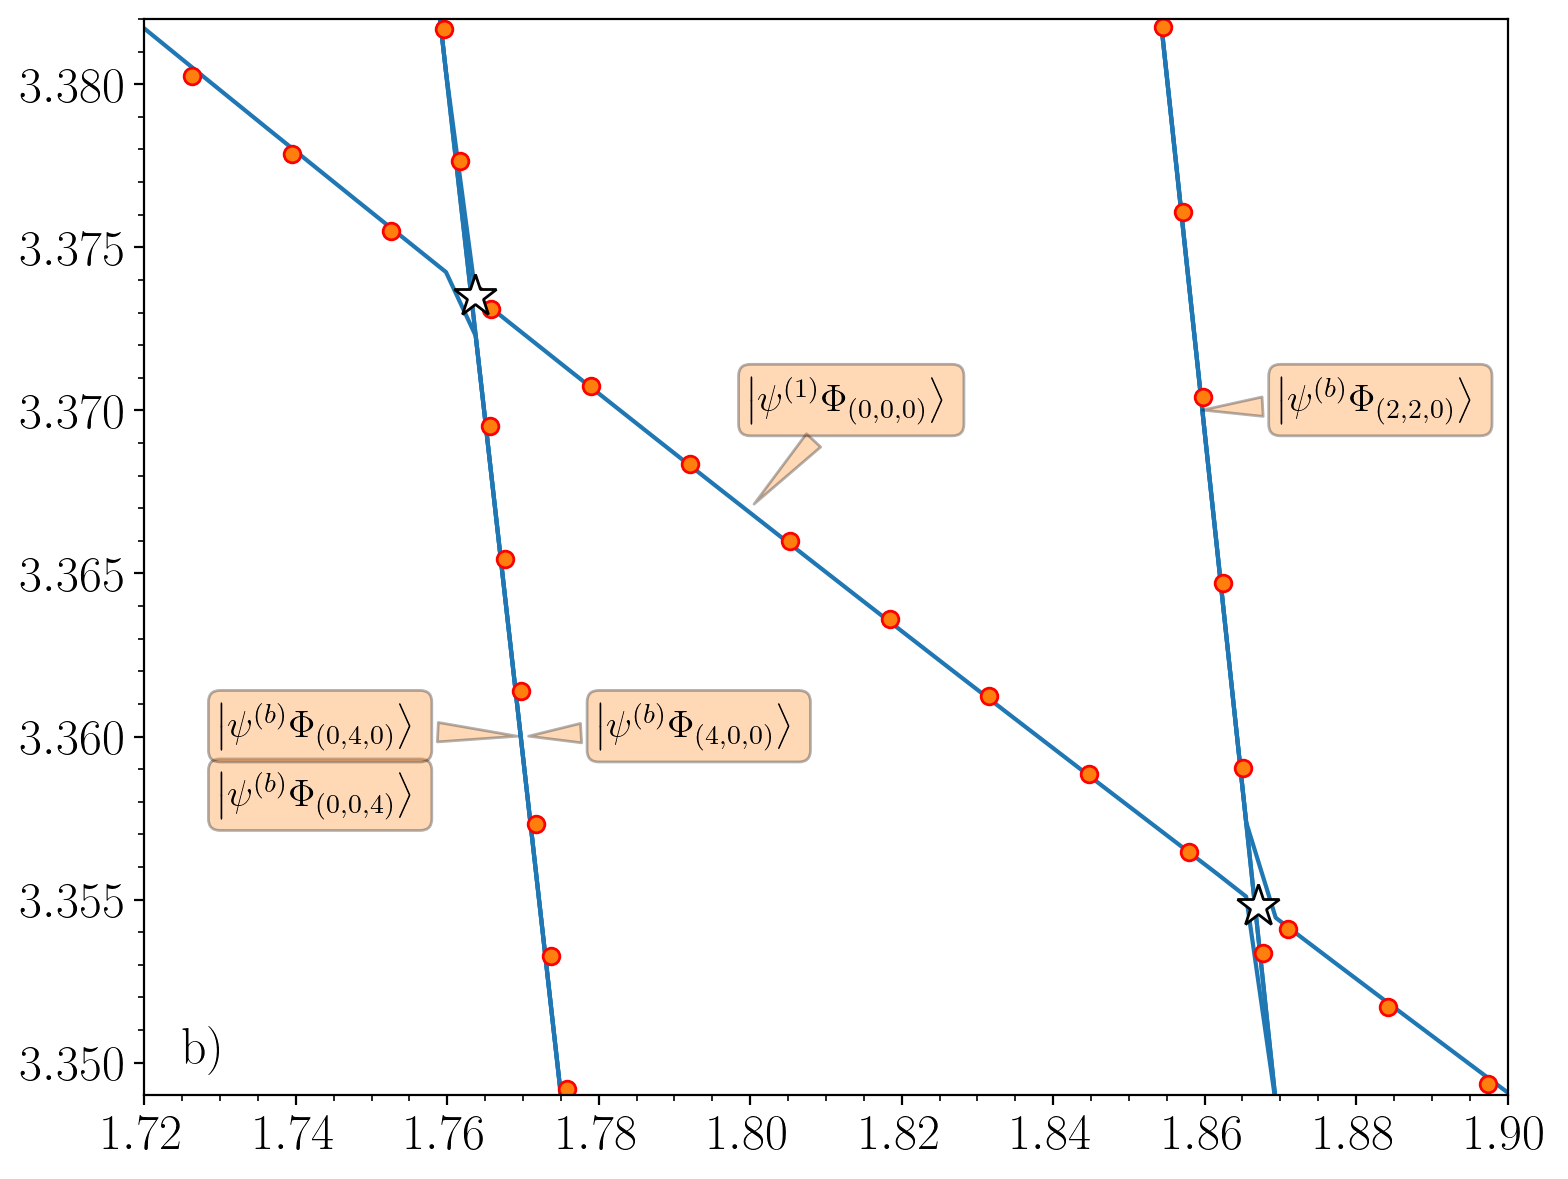
\includegraphics[scale=0.30]{/Users/tomy/PhD/Ultracold_Atoms_src/Analysis/q3d/Results/Figures/Ix4993_Iy4993_Iz4993_Easc_Interpolation_v2.png}
    	\caption{Zoom to the Inelastic CIR which arises from the avoided crossings between the first trap state and the transversally excited bound states. Diabatic states responsible of Inelastic CIR are drawn with red dashed lines and labeled by kets. For anisotropic transversal confinement the CIR splits in two due to the symmetry breaking.}
    	\label{fig:Isotropic Crossings}
	\end{figure}
	
	\begin{figure}[H]
	 \begin{subfigure}{0.5\textwidth}
	  \centering
	 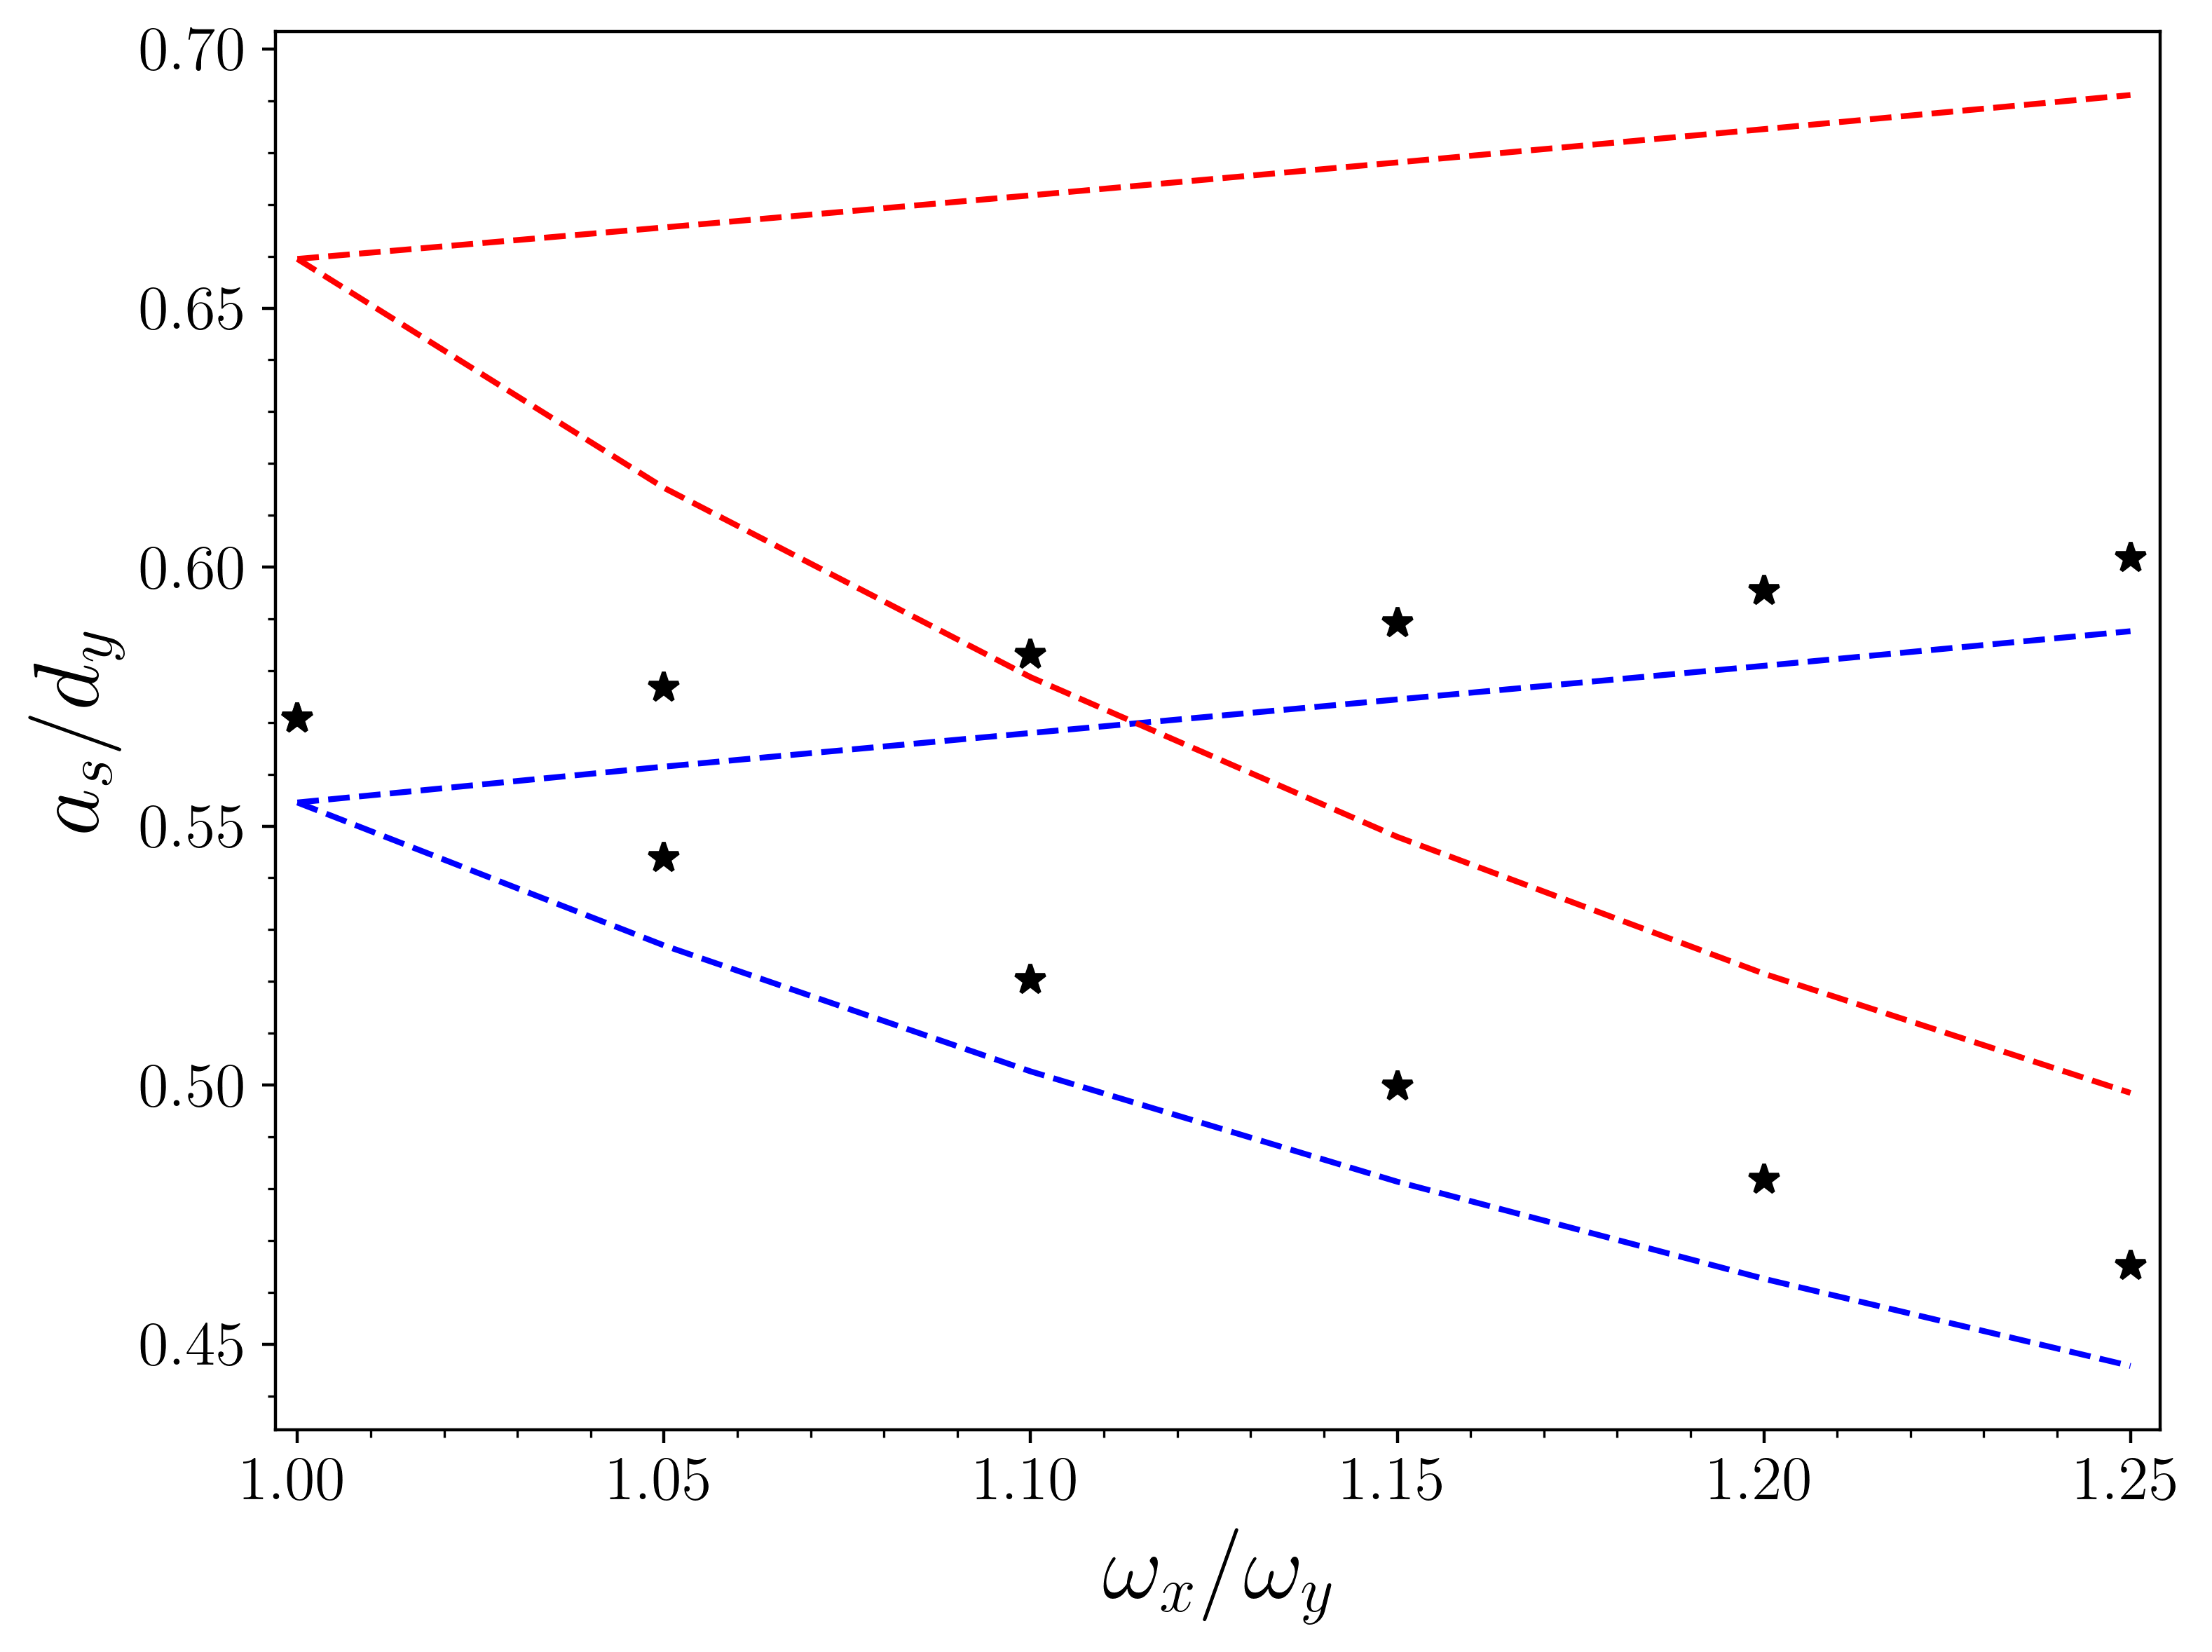
\includegraphics[scale=0.30]{/Users/tomy/PhD/Ultracold_Atoms_src/Analysis/q3d/Results/Figures/ICIR_q3D_Theory_Comparison.png}
	 \end{subfigure}
	 \vspace{10pt}
	 \begin{subfigure}{0.5\textwidth}
	   \centering
    	 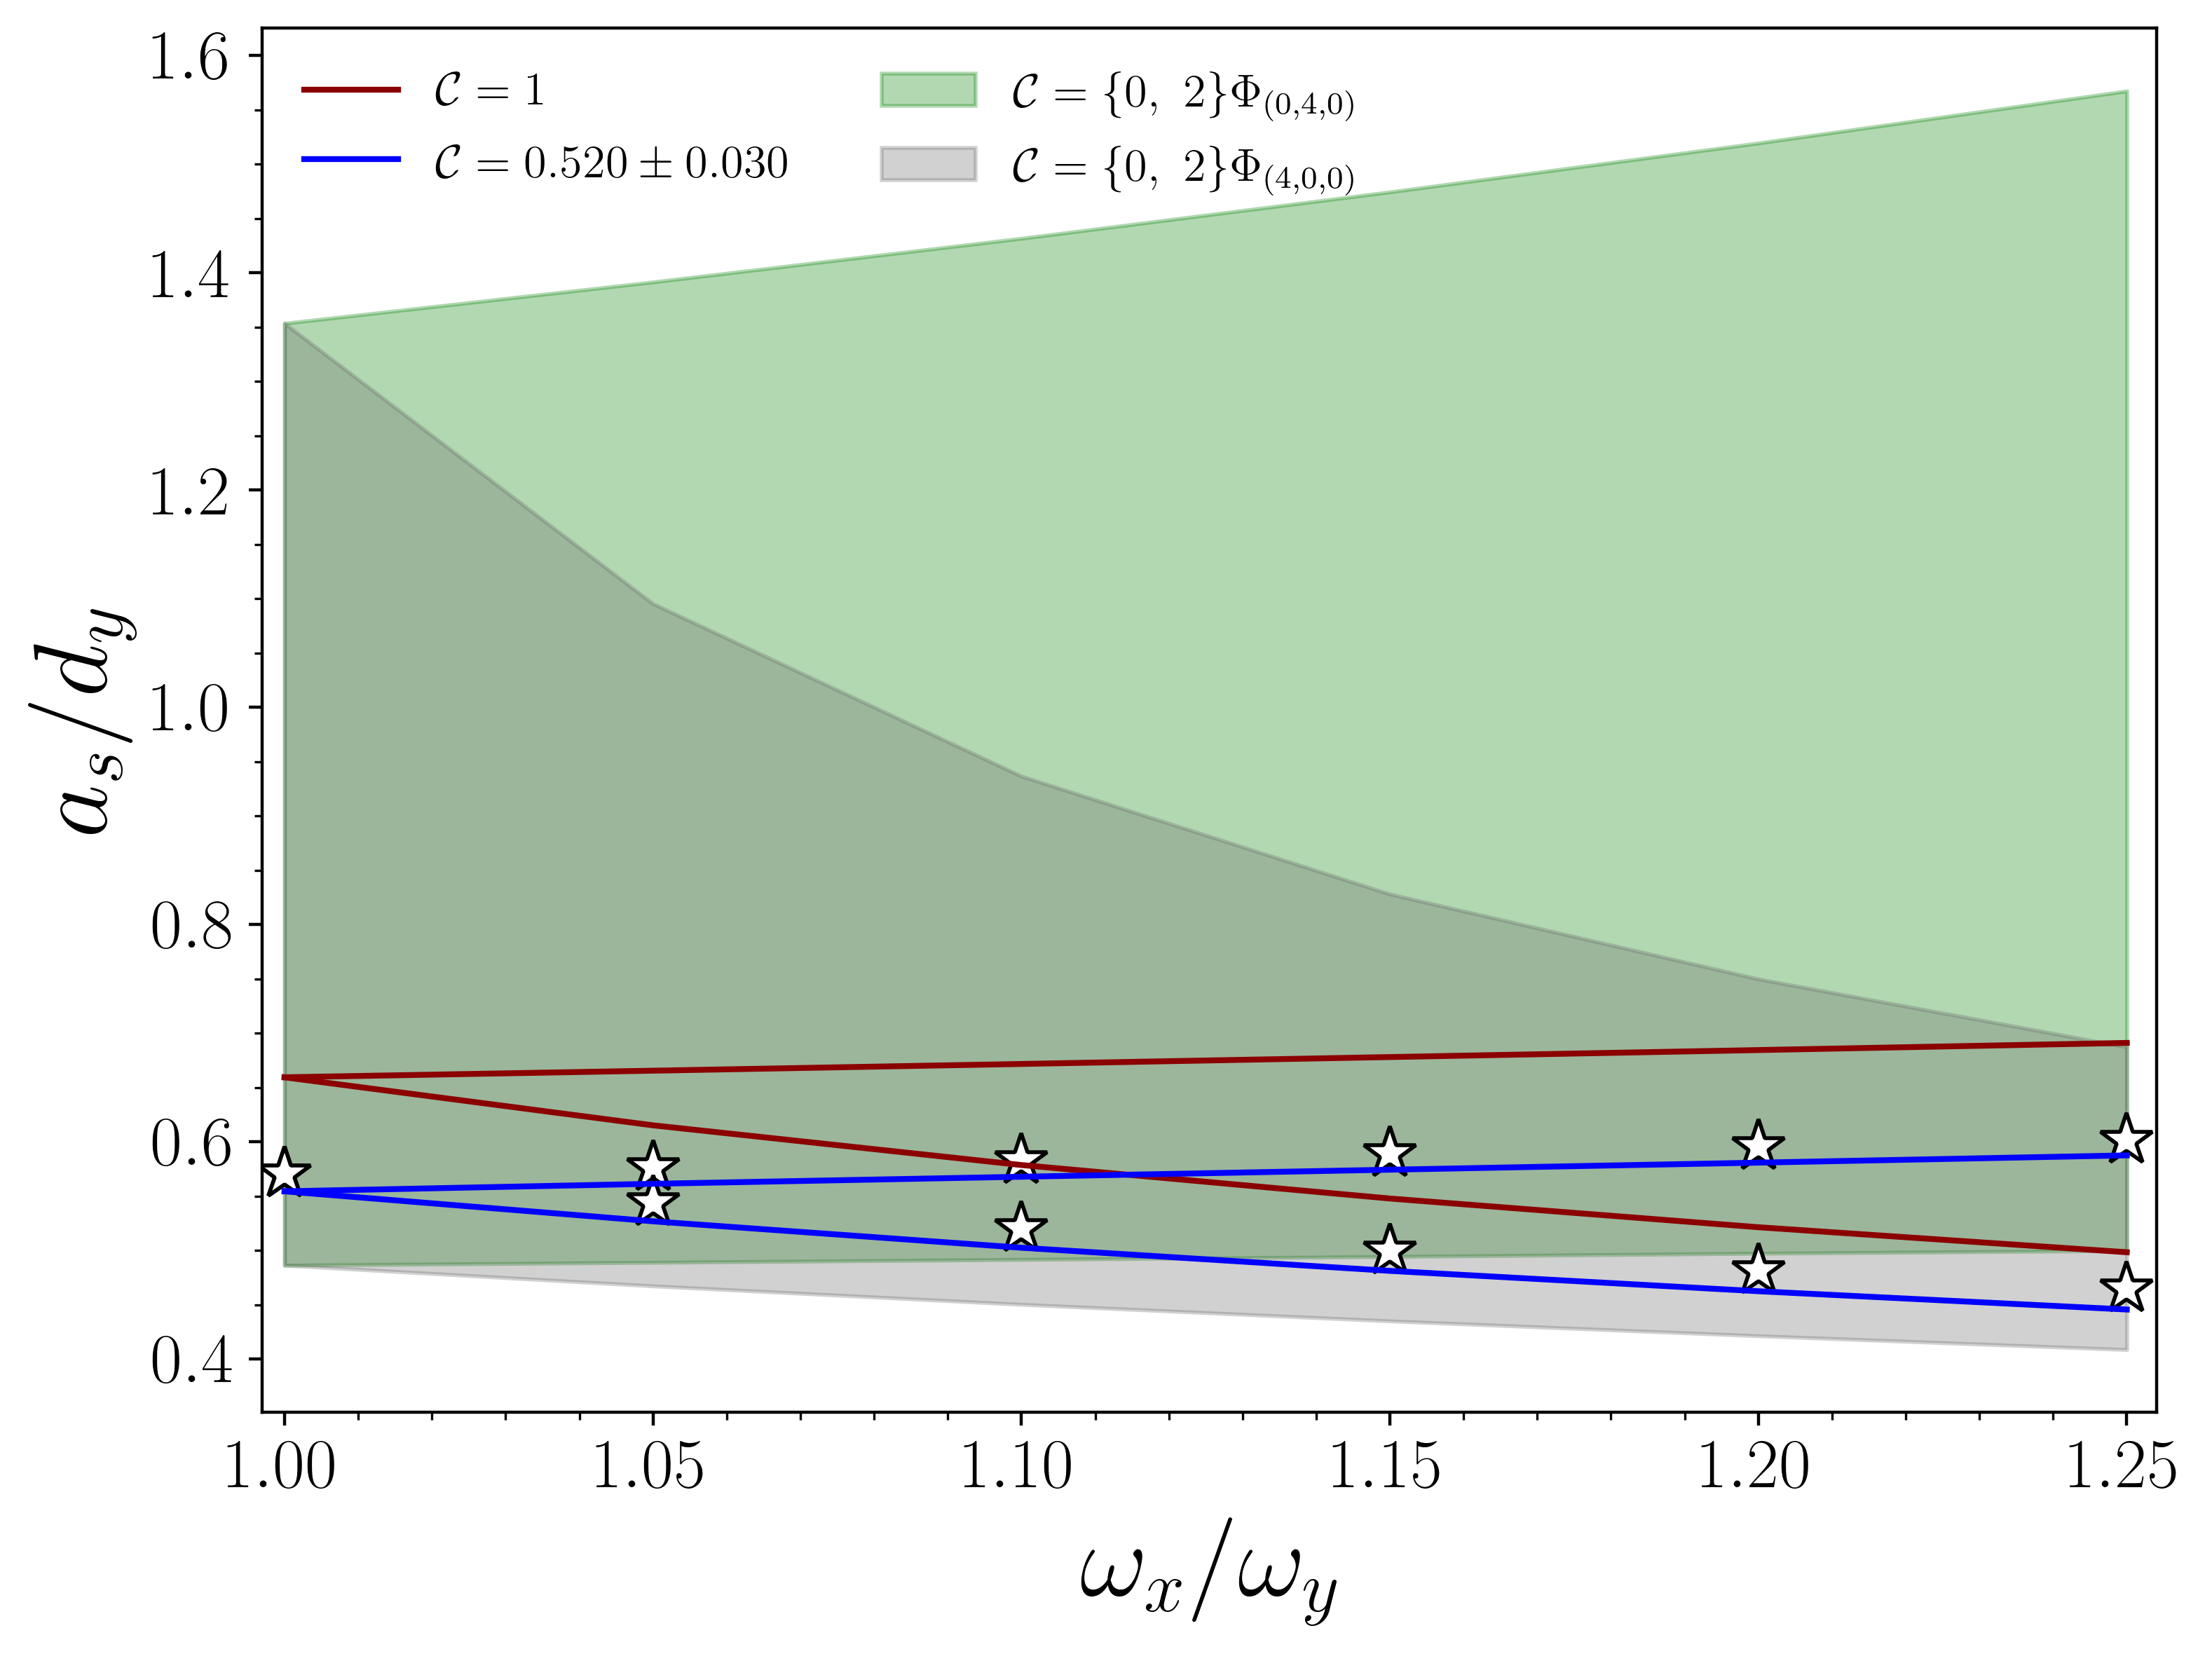
\includegraphics[scale=0.30]{/Users/tomy/PhD/Ultracold_Atoms_src/Analysis/q3d/Results/Figures/ICIR_q3D_Theory_band.png}
	 \end{subfigure}
    	\caption{Positions of the four excitations Inelastic CIR in terms of the characteristic transversal length for different values of transversal anisotropy in 3-D. Black stars are the ab initio calculations, blue dashed lines the exact theory computations with a constant $C=0.52\pm0.03$, red dashed lines $C=1$ and gray shadows the corresponding theory computations with both $C=2$ and $C=0$. }
    	\label{fig:q3d ICIR}
	\end{figure}
	
	%\begin{figure}[H]
%\centering
%\subfigure{\includegraphics[width=8cm, %height=6cm]{Union/dL(z)u.png}}\hspace{0.5mm}
%\subfigure{\includegraphics[width=8cm, height=6cm]{Golf/dL(z)g.png}}
%\label{Figura 1}
%\caption{M�dulo de distancias respecto al redshift para los datos de Union (izquierda) y Gold (derecha).}
%\end{figure}

%------------------------------------------------------------------------------------
\subsection{quasi 1-D}
\begin{figure}[H]
   	 \centering
    	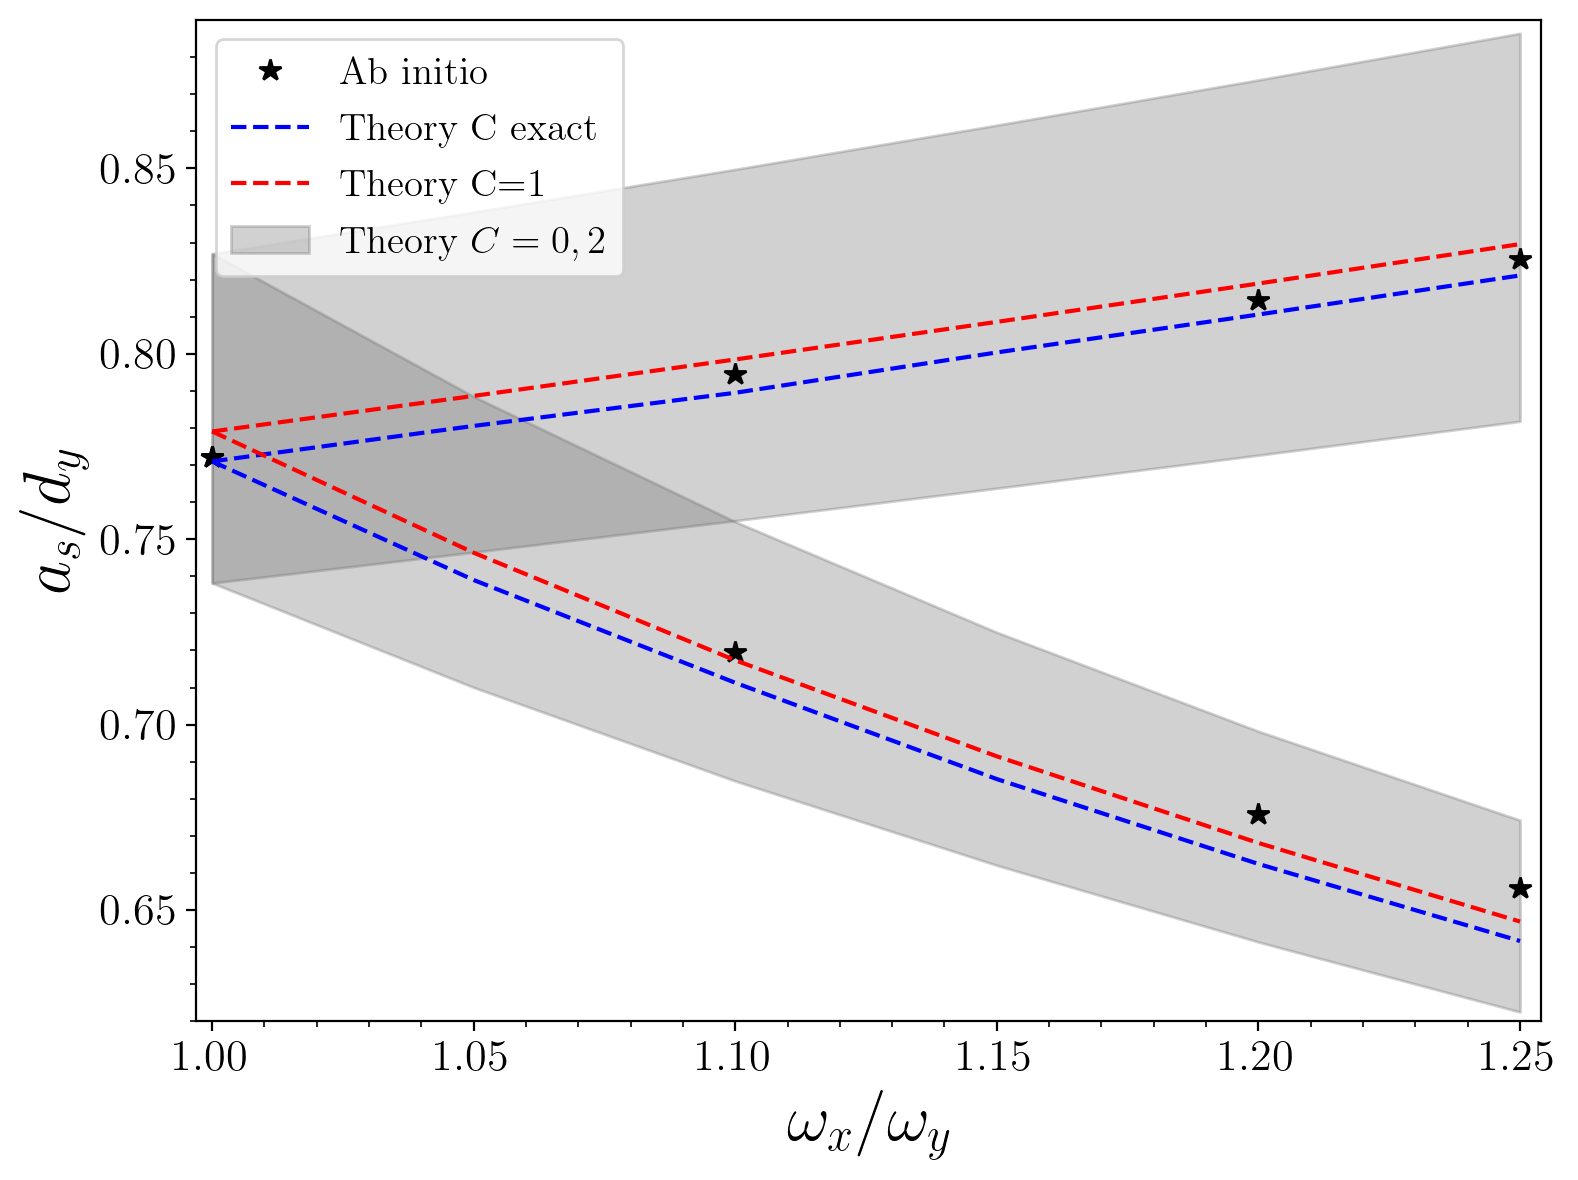
\includegraphics[scale=0.30]{/Users/tomy/PhD/Ultracold_Atoms_src/Analysis/q1d/Results/Figures/ICIR_q1D_Theory_band_coupling.png}
    	\caption{Positions of the two-excitations Inelastic CIR in terms of the characteristic transversal length for different values of transversal anisotropy in 3-D. Black stars are the ab initio calculations, blue dashed lines the exact theory computations with a constant $C=0.52\pm0.03$, red dashed lines $C=1$ and gray shadows the corresponding theory computations with both $C=2$ and $C=0$.}
    	\label{fig:q1D ICIR}
	\end{figure}

%------------------------------------------------------------------------------------
\section{Origin of the asymmetric splitting of the Inelastic CIR} \label{sec:perturbation}
Contar teoría de perturbaciones y lo que hizo Fabio

%------------------------------------------------------------------------------------
\section{Conclusions}
%------------------------------------------------------------------------------------
\section*{Anknowledgements}
%------------------------------------------------------------------------------------
\section*{References}
\bibliographystyle{unsrtnat}
\bibliography{q1d_q3d_perturbationCitation.bib}

\newpage

\end{document}

















